% file: DGDT_dump.tex
% Differential Geometry, Differential Topology, in unconventional ``grande'' format; fitting a widescreen format
% 
% github        : ernestyalumni
% linkedin      : ernestyalumni 
% wordpress.com : ernestyalumni
%
% This code is open-source, governed by the Creative Common license.  Use of this code is governed by the Caltech Honor Code: ``No member of the Caltech community shall take unfair advantage of any other member of the Caltech community.'' 
% 

\documentclass[10pt]{amsart}
\pdfoutput=1
\usepackage{mathtools,amssymb,lipsum,caption}

\usepackage{graphicx}
\usepackage{hyperref}
\usepackage[utf8]{inputenc}
\usepackage{listings}
\usepackage[table]{xcolor}
\usepackage{pdfpages}
%\usepackage[version=3]{mhchem}
\usepackage{mhchem}

\usepackage{tikz}
\usetikzlibrary{matrix,arrows}

\usepackage{multicol}

\hypersetup{colorlinks=true,citecolor=[rgb]{0,0.4,0}}

\oddsidemargin=15pt
\evensidemargin=5pt
\hoffset-45pt
\voffset-55pt
\topmargin=-4pt
\headsep=5pt
\textwidth=1120pt
\textheight=595pt
\paperwidth=1200pt
\paperheight=700pt
\footskip=40pt








\newtheorem{theorem}{Theorem}
\newtheorem{corollary}{Corollary}
%\newtheorem*{main}{Main Theorem}
\newtheorem{lemma}{Lemma}
\newtheorem{proposition}{Proposition}

\newtheorem{definition}{Definition}
\newtheorem{remark}{Remark}

\newenvironment{claim}[1]{\par\noindent\underline{Claim:}\space#1}{}
\newenvironment{claimproof}[1]{\par\noindent\underline{Proof:}\space#1}{\hfill $\blacksquare$}

%This defines a new command \questionhead which takes one argument and
%prints out Question #. with some space.
\newcommand{\questionhead}[1]
  {\bigskip\bigskip
   \noindent{\small\bf Question #1.}
   \bigskip}

\newcommand{\problemhead}[1]
  {
   \noindent{\small\bf Problem #1.}
   }

\newcommand{\exercisehead}[1]
  { \smallskip
   \noindent{\small\bf Exercise #1.}
  }

\newcommand{\solutionhead}[1]
  {
   \noindent{\small\bf Solution #1.}
   }


\title{The Differential Geometry Differential Topology Dump}
\author{Ernest Yeung \href{mailto:ernestyalumni@gmail.com}{ernestyalumni@gmail.com}}
\date{28 juillet 2016}
\keywords{Differential Geometry, Differential Topology}
\begin{document}

\definecolor{darkgreen}{rgb}{0,0.4,0}
\lstset{language=Python,
 frame=bottomline,
 basicstyle=\scriptsize,
 identifierstyle=\color{blue},
 keywordstyle=\bfseries,
 commentstyle=\color{darkgreen},
 stringstyle=\color{red},
 }
%\lstlistoflistings

\maketitle



\begin{multicols*}{2}

  
\setcounter{tocdepth}{1}
\tableofcontents



\begin{abstract}
Everything about Differential Geometry, Differential Topology

\end{abstract}

\part{}


\section{Inverse Function Theorem}

Shastri (2011) had a thorough and lucid and explicit explanation of the Inverse Function Theorem \cite{AShastri2011}.  I will recap it here.  The following is also a blend of Wienhard's Handout 4 \url{https://web.math.princeton.edu/~wienhard/teaching/M327/handout4.pdf}

\begin{definition}
  Let $(X,a)$ metric space.  

\textbf{contraction} $\phi:X \to X$ if $\exists \, $ constant $0<c<1$ s.t. $\forall \, x,y \in X$
\[
d(\phi(x),\phi(y)) \leq cd(x,y)
\]
\end{definition}

\begin{theorem}[Contraction Mapping Principle]
  Let $(X,d)$ complete metric space.  \\
Then $\forall \, $ contraction $\phi:X\to X$, $\exists \, ! y\in X$ s.t. $\phi(y) = y$, $y$ \emph{fixed pt.}
\end{theorem}

\begin{proof}
  Recall def. of complete metric space $X$, $X$ metric space s.t. $\forall \, $ Cauchy sequence in $X$ is convergent in $X$ (i.e. has limit in $X$).  

$\forall \, x_0 \in X$,
Define $\begin{aligned} & \quad \\
  & x_1 = \phi(x_0) \\ 
  & x_2 = \phi(x_1) \\ 
  & \vdots \\
  & x_j = \phi(x_{j-1}) \\ 
  & \vdots \\
  & x_n = \phi(x_{n-1})
\end{aligned}$

\[
\begin{gathered}
  d(x_{n+1},x_n) = d(\phi(x_n),\phi(x_{n-1})) \leq c d(x_n,x_{n-1}) \leq \dots \leq c^nd(x_1,x_0)
\end{gathered}
\]
for some $0< c<1$.

\[
d(x_m,x_n) \leq d(x_n,x_{n-1}) + d(x_{n-1},x_m) \leq d(x_n,x_{n-1}) + d(x_{n-1},x_{n-2}) + \dots + d(x_{m+1},x_m) \leq \sum_{k=n-1}^m c^k d(x_1,x_0)
\]
Thus, $\forall \, \epsilon >0$, $\exists \, n_0 >0$, ($n_0$ large enough) s.t. $\forall \, m ,n\in \mathbb{N}$ s.t. $n_0 < n <m$, 
\[
d(x_m,x_n) \leq \sum_{k=n-1}^m c^k d(x_1,x_0) < \epsilon d(x_1,x_0)
\]
Thus, $\lbrace x_n \rbrace$ Cauchy sequence.  Since $X$ complete, $\exists \, $ limit pt. $y \in X$ of $\lbrace x_n \rbrace$.  
\[
\phi(y) = \phi(\lim_n x_n) = \lim_n \phi(x_n) = \lim_n x_{n+1} = y
\]
Since by def. of $y$ limit pt. of $\lbrace x_n \rbrace$, $\forall \, \epsilon >0$, then $\lbrace n | |x_n -y|\leq \epsilon, \, n \in \mathbb{N}\rbrace$ is infinite.  

Consider $\delta > \mathbb{N}$.  Consider $\lbrace n | |x_n-y| \leq \delta, n \in \mathbb{N}\rbrace$ 

$\exists \, N_{\delta} \in \mathbb{N}$ s.t. $\forall \, n > N_{\delta}$, $|x_n-y|< \delta$; otherwise, $\forall \, N_{\delta}$, $\exists \, n > N_{\delta}$ s.t. $|x_n - y| \geq \delta$.  Then $\lbrace n | |x_n -y| \leq \delta , n \in \mathbb{N} \rbrace$ finite.  Contradiction.  

$\phi$ cont. so by def. $\forall \, \epsilon >0$, $\exists \, \delta >0$ s.t. if $|x_n -y| < \delta$, then $|\phi(x_n) - \phi(y) | < \epsilon$.  

Pick $N_{\delta}$ s.t. $\forall \, n > N_{\delta}$, $|x_n-y| < \delta$, and so $|\phi(x_n) - \phi(y)|< \epsilon$. There are infinitely many $\phi(x_n)$'s that satisfy this, and so $\phi(y)$ is a limit pt.  

If $\exists \, y_1,y_2 \in X$ s.t. $\begin{aligned} & \quad \\
  & \phi(y_1) = y_1 \\ 
  & \phi(y_2) = y_2 \end{aligned}$, then
\[
d(y_1,y_2) = d(\phi(y_1), \phi(y_2)) \leq c d(y_1,y_2) \text{ with } c <1
\]
so $c=1$
\end{proof}


\begin{theorem}[Inverse Function Theorem]
  Suppose open $U \subset \mathbb{R}^n$, let $C^1 \, f: U \to \mathbb{R}^n$, $x_0 \in U$ s.t. $Df(x_0)$ invertible.  

%  Let open $E \subset \mathbb{R}^n$, $0 \subset E$, let $f \in \mathcal{C}^1(E,\mathbb{R}^n)$ s.t. $Df(0)$ invertible.  

Then $\exists \,$ open neighborhoods $V\ni x_0$, $W \ni f(x_0)$ s.t. $V\subseteq U$ and $W\subseteq \mathbb{R}^n$, respectively, and s.t.

\begin{enumerate}
\item[(i)] $f: V\to W$ bijection
\item[(ii)] $g = f^{-1}:V \to U$ differentiable, i.e. $g = f^{-1}:W\to V$ is $C^1$
\item[(iii)] $D(f^{-1}) $ cont. on $W$.  
\item[(iv)] $Dg(y) = (Df(g(y)))^{-1}$ \, $\forall \, y \in W$
\end{enumerate}
Also, notice that $f(g(y)) = y \, \forall \, y \in W$.  
\end{theorem}

\begin{proof}
%  Let $A = Df(0)$, consider $\widehat{f} = A^{-1}\circ f$.  Then $\widehat{f} \in (U;\mathbb{R}^n)$.  $D(\widehat{f})(0)=1$ since $D(\widehat{f})(0) = D(A^{-1} \circ f)(0)=A^{-1}Df(0)=1$.  

Consider $\widetilde{f}(x) = (Df(x_0))^{-1}(f(x+x_0) - f(x_0))$.  Then \\
\phantom{Consider} $\widetilde{f}(0) = 0$ and 
\[
\begin{aligned}
  &  D\widetilde{f}= (Df(x_0))^{-1}(Df(x+x_0) -0)  \\
  & D\widetilde{f}(0) = (Df(x_0))^{-1}Df(x_0)=1
\end{aligned}
\]  
So let $\widetilde{f}\to f$ (notation) and so assume, without loss of generality, that $U\ni 0$, $f(0)=0$, $Df(0)=1$

Choose $0 < \epsilon \leq \frac{1}{2}$.  Let $0< \delta <1$ s.t. open ball $V = B_{\delta}(0) \subseteq U$, and $\| Df(x)-1\| < \epsilon$.  $\forall \, x \in U$, since $Df$ cont. at $0$.  

Let $W=f(V)$.  

$\forall \, y \in W$, define $\begin{aligned} & \quad \\
  & \phi_y : V \to \mathbb{R}^n \\
  & \phi_y(x) = x + (y-f(x))\end{aligned}$

\[
\begin{aligned}
  & D(\phi_y)(x) = 1 + - Df(x) \quad \, \forall \, x \in V \\ 
  & \| D(\phi_y)(x) \| = \| 1 - Df(x) \| \leq \epsilon <1
\end{aligned}
\]

$\forall \, x_1 ,x_2 \in V$, by mean value Thm. (not the equality that is only valid in 1-dim., but the inequality, that's valid for $\mathbb{R}^d$, 
\[
\| \phi_y(x_1) - \phi_y(x_2) \| \leq \| D(\phi_y)(x') \| \| x_1 - x_2 \| 
\]
for some $x' = cx_2 + (1-c)x_1$, $c\in [0,1]$.  $V$ only needed to be convex set.  
\[
\Longrightarrow \| \phi_y(x_1) - \phi_y(x_2) \| \leq \epsilon \| x_1 - x_2 \|
\]
Then $\phi_y$ contraction mapping.  

Suppose $f(x_1) = f(x_2)=y$, $x_1,x_2 \in V$.  
\[
\begin{gathered}
\begin{aligned}
  & \phi_y(x_1) =x_1 \\ 
  & \phi_y(x_2) =x_2  
\end{aligned} \\
\| \phi_y(x_1) - \phi_y(x_2) \| = \| x_1 - x_2 \| \leq \epsilon \| x_1 - x_2 \| \quad \, \forall \, \epsilon > 0 \Longrightarrow x_1 = x_2 
\end{gathered}
\]
$\Longrightarrow \left. f\right|_U$ injective.

$W=f(V)$, so $f:V\to W$ surjective.  $f$ bijective.  

Fix $y_0 \in W$, $y_0 = f(x_0)$, $x_0 \in V$.  \\
Let $r>0$ s.t. $B_r(x_0) \subset V$.  \\
Consider $B_{r\epsilon}(y_0)$.  If $y\in B_{r\epsilon}(y_0)$.  
\[
\begin{gathered}
  r\epsilon > \| y-y_0 \| = \| y - f(x_0) \| = \| \phi_y(x_0) - x_0 \| \text{ with } \\
  \phi_y(x) = x + (y-f(x))
\end{gathered}
\]

If $x\in B_r(x_0)$, 
\[
\| \phi_y(x) -x_0 \| \leq \| \phi_y(x) - \phi_y(x_0) \|  + \| \phi_y(x_0) - x_0 \| \leq \epsilon \| x-x_0 \| + r\epsilon < 2 r\epsilon = r
\]

%Consider $B_{r\epsilon }(y_0)$.  

Thus $\phi(B_r(x_0)) = B_r(x_0)$.

By contraction mapping principle, $\exists \, a \in B_r(x_0)$, s.t. $\phi_y(a)=a$.  Then $\phi_y(a) = a+ (y-f(a)) = a \Longrightarrow f(a) =y$.  

$y\in f(V) = W$.  

So $B_{r\epsilon}(y_0) \subset W$.  $W$ open.  

Let $\text{Mat}(n,n) \equiv $ space of all $n\times n$ matrices; $\text{Mat}(n,n)  = \mathbb{R}^{n^2}$.  


\end{proof}

There is a proof of the implicit function theorem and its various forms in Shastri (2011) \cite{AShastri2011}, but I found Wienhard's Handout 4 for Math 327 to be clearer.\footnote{\url{https://web.math.princeton.edu/~wienhard/teaching/M327/handout4.pdf}}

\begin{theorem}[Implicit Function Theorem]
Let open $U \subset \mathbb{R}^{m+n} \equiv \mathbb{R}^m \times \mathbb{R}^n$  \\
\phantom{Let} $C^1 \, f:U \to \mathbb{R}^n $ \\
\phantom{Let} $(a,b) \in U$ s.t. $f(a,b) = 0$ and $\left. D_y f\right|_{(a,b)}$ invertible.  

Then $\exists \, $ open $V \ni (a,b)$, $V \subset U$ \\
\phantom{Then} $\exists \, $ open neighborhood $W \ni a$, $W \subseteq \mathbb{R}^m$ \\
\phantom{Then} $\exists \, !$ \, $C^1 \, g:W \to \mathbb{R}^n$ s.t.
\[
\lbrace (x,y) \in V | f(x,y) =0 \rbrace = \lbrace (x,g(x)) | x \in W \rbrace
\]
Moreover,
\[
dg_x = - \left. (d_yf)^{-1} \right|_{(x,g(x))} \left. d_x f\right|_{(x,g(x))}
\]
and $g$ smooth if $f$.  
\end{theorem}

\begin{proof}
  Define $\begin{aligned} & \quad \\
    & F: U \to \mathbb{R}^{m+n}   \\
    & F(x,y) = (x,f(x,y)) \end{aligned}$

Then $F(a,b) = (a,0)$ (given), and 
\[
DF = \left[ \begin{matrix} 1 & \\ 
    \frac{ \partial f^i(x,y)}{ \partial x^j} & \frac{ \partial f^i(x,y) }{ \partial y^j } \end{matrix} \right] \equiv \left[ \begin{matrix} 1 & \\
    D_xf & D_yf \end{matrix} \right]
\]
$DF(a,b)$ invertible.  

By inverse function theorem, since $DF(a,b)$ invertible at pt. $(a,b)$, \\
$\exists \, $ open neighborhoods $\begin{aligned} & \quad \\
  & V \ni (a,b) \subseteq \mathbb{R}^m \times \mathbb{R}^n \\
  & \widetilde{W} \ni (a,0) \subseteq \mathbb{R}^m \times \mathbb{R}^n \end{aligned}$ s.t. $F$ diffeomorphism with $F^{-1}: \widetilde{W} \to V$. 

Set $W = \lbrace x \in \mathbb{R}^m | (x,0) \in \widetilde{W}\rbrace$.  Then $\pi_1(\widetilde{W}) =W$ open in $\mathbb{R}^m$.  

Define $g:W\to \mathbb{R}^n$, 
\[
\begin{aligned}
  & g(x) = \pi_2 \circ F^{-1}(x,0) \text{ or } \\ 
  & F^{-1}(x,0) = (h(x),g(x))
\end{aligned}
\]

Now $FF^{-1}(x,0) = (x,0) = (h(x), f(h(x),g(x)) )$ so $h(x)=x \, \forall \, x \in W$, $0 = f(x,g(x))$.  

Then
\[
\lbrace (x,y) \in V | f(x,y) = 0 \rbrace = \lbrace (x,y) \in V | F(x,y) = (x,0) \rbrace = \lbrace (x,g(x)) | x \in W, 0 = f(x,g(x)) \rbrace
\]
Since $\pi$ smooth and $F^{-1}$ is $C^1$, $g$ is $C^1$.  

To reiterate, $f(x,g(x)) =0$ on $W$.

Using chain rule while differentiating $f(x,g(x))=0$, 
\[
\begin{gathered}
\partial_{x^j} f(x,g(x)) = \frac{ \partial f(x,g(x)) }{ \partial x^k} \frac{ \partial x^k}{ \partial x^j}+ \frac{ \partial f(x,g(x))}{ \partial y^k}\frac{ \partial g^k(x)}{\partial x^j} = \left. D_x f \right|_{(x,g(x))} + \left. (D_yf) \right|_{(x,g(x))} \cdot (Dg)_x = 0 \text{ or }  \\
(Dg)_x = -\left. (D_yf) \right|_{x,g(x)} \left. D_xf \right|_{(x,g(x))}
\end{gathered}
\]



\end{proof}

\begin{definition}
  smooth $f:M \to N$, s.t. $Df(p) : T_pM \to T_{f(p)}N$ injective.  Then $f$ immersion at $p$.  
\end{definition}

Shastri (2011) has this as the ``Injective Form of Implicit Function Theorem'', Thm. 1.4.5, pp. 23 and Guillemin and Pollack (2010) has this as the ``Local Immersion Theorem'' on pp. 15, Section 3 ``The Inverse Function Theorem and Immersions'' \cite{VGuilleminAPollack2010}.  

\begin{theorem}[Local immersion Theorem i.e. Injective Form of Implicit Function Theorem]
  Suppose $f:M\to N$ immersion at $p$, $q=f(p)$.  

Then $\exists \, $ local coordinates around $p,q$, $x,y$, respectively s.t. $f(x_1\dots x_m) = (x_1 \dots x_m,0 \dots 0)$.  

\end{theorem}

\begin{proof}
  Choose local parametrizations 
\[
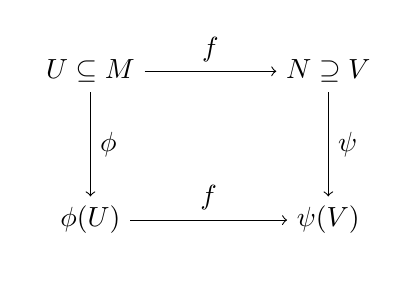
\begin{tikzpicture}
  \matrix (m) [matrix of math nodes, row sep=3.8em, column sep=4.8em, minimum width=2.2em]
  {
    U \subseteq M & N \supseteq V \\
    \phi(U) & \psi(V) \\
};
  \path[->]
  (m-1-1) edge node [above] {$f $} (m-1-2)
          edge node [auto] {$\phi$} (m-2-1)
  (m-1-2) edge node [auto]  {$\psi$} (m-2-2)
  (m-2-1) edge node [auto] {$f$} (m-2-2)
  ;
\end{tikzpicture}  
\quad \quad \, \begin{aligned} & \phi(p) = x \\
  & \psi(q) = y \end{aligned}
\]
$D(\psi f\varphi^{-1}) \equiv Df$.  $Df(p)$ injective (given $f$ immersion).  $Df(p) \in \text{Mat}(n,m)$

By change of basis in $\mathbb{R}^n$, assume $Df(p) = \left( \begin{matrix} I_m \\ 0 \end{matrix} \right)$.  

Now define $\begin{aligned} & \quad \\
  & G : \phi(U) \times \mathbb{R}^{n-m} \to \mathbb{R}^n \\
  & G(x,z) = f(x) + (0,z) \end{aligned}$

Thus, $DG(x,z) =1$ and for open $\phi(U) \times U_2$, $ G(\phi(U)\times U_2)$ open.  

By inverse function theorem, $G$ local diffeomorphism of $\mathbb{R}^n$, at $0$.  

Now $f = G\circ \mathfrak{i}$, where $\mathfrak{i}$ is canonical immersion.  
\[
\begin{gathered}
  G(x,0) = f(x) \\
  \Longrightarrow G^{-1}G(x,0) = (x,0) = G^{-1}f(x)
\end{gathered}
\]

Use $\psi \circ G$ as the local parametrization of $N$ around pt. $q$.  Shrink $U,V$ so that 

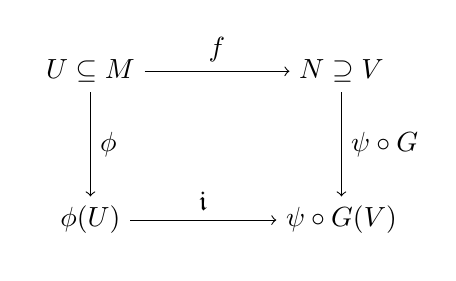
\begin{tikzpicture}
  \matrix (m) [matrix of math nodes, row sep=3.8em, column sep=4.8em, minimum width=2.2em]
  {
    U \subseteq M & N \supseteq V \\
    \phi(U) & \psi\circ G(V) \\
};
  \path[->]
  (m-1-1) edge node [above] {$f $} (m-1-2)
          edge node [auto] {$\phi$} (m-2-1)
  (m-1-2) edge node [auto]  {$\psi\circ G$} (m-2-2)
  (m-2-1) edge node [auto] {$\mathfrak{i}$} (m-2-2)
  ;
\end{tikzpicture}  

\end{proof}






\begin{theorem}[(Implicit Function Thm.)]
  Let open subset $U\subseteq \mathbb{R}^n \times \mathbb{R}^d$, $(x,y) = (x^1 \dots x^n, y^1 \dots y^k) $ on $U$.  \\
  Suppose smooth $\Phi:U\to \mathbb{R}^k$, $(a,b) \in U$, $c=\Phi(a,b)$

  If $k\times k$ matrix $\frac{ \partial \Phi^i}{ \partial y^j}(a,b)$ nonsingular, then $\exists $ neighborhoods $\begin{aligned} & \quad \\
    & V_0 \subseteq \mathbb{R}^n \text{ of $a$ } \\
    & W_0 \subseteq \mathbb{R}^k \text{ of $b$ } \end{aligned}$ and smooth $F:V_0 \to W_0$ s.t.

  $\Phi^{-1}(c) \bigcap (V_0\times W_0)$ is graph of $F$, i.e. \\
  $\Phi(x,y) =c$ for $(x,y) \in V_0\times W_0$ iff $y=F(x)$.  
  \end{theorem}



Jeffrey Lee (2009) \cite{JLee2009}



John Lee (2012) \cite{JLee2012}


\part{Pr\'{a}staro}

Pr\'{a}staro (1996) \cite{Pras1996}

\subsubsection{Affine Spaces}

cf. Sec. 1.2 - \emph{Affine Spaces} of Pr\'{a}staro (1996) \cite{Pras1996}

\begin{definition}[affine space]
  \begin{equation}
\begin{gathered}
    \text{ affine space \qquad \, } (M, \mathbf{M}, \alpha )  \\
    \text{ with } \\
    \begin{aligned}
      & M \equiv \text{ set (set of pts.) }  \\ 
      & \mathbf{M} \equiv \text{ vector space (space of free vectors) } \\
      & \alpha \equiv \mathbf{M} \times M \to M \equiv \text{ translation operator } \\
      & \alpha : (v,p ) \mapsto p' \equiv p + v
      \end{aligned}
\end{gathered}
  \end{equation}
  Note: $\alpha$ is a \textbf{transitive} action and without fixed pts. (free).

  i.e. $\forall \, p \in M$, 
  \end{definition}

$\forall \, $ pt. $O \in M$, $\alpha:(v,O) \mapsto O' \equiv O + v$, $\alpha (\cdot , O) \equiv \alpha_O \equiv \alpha(O)$.  $\alpha_O(v) = O' = O + \mathbf{v}$ \qquad \, $\forall \, O' \in M$, $\exists \, \mathbf{v} \in \mathbf{M}$ s.t. $O' = O + \mathbf{v}$ \\
$\Longrightarrow M \equiv \mathbf{M}$.

$\forall \, (O, \lbrace e_i \rbrace)_{1 \leq i \leq n }$, where $\lbrace e_i \rbrace$ basis of $\mathbf{M}$, $M \equiv \mathbf{M} = \mathbb{R}^n$ so isomorphism $M \simeq \mathbb{R}^n$ \\
\begin{definition}
  $(O, \lbrace e_i \rbrace) \equiv $ affine frame.

  $\forall \, $ affine frame $(O,\lbrace e_i \rbrace)$, $\exists \, $ coordinate system $x^{\alpha} : M \to \mathbb{R}$, \\
  where $x^{\alpha}(p)$ is $\alpha$th component, in basis $\lbrace e_i \rbrace$, of vector $p-O$
  \end{definition}

\begin{theorem}[1.4 Pr\'{a}staro (1996) \cite{Pras1996}]
  Let $(x^{\alpha}), (\overline{a}^{\alpha})$ 2 coordinate systems correspond to affine frames $(O, \lbrace e_i \rbrace)$, $( \overline{O}, \lbrace \overline{e}_i \rbrace )$, respectively.
\begin{equation}
  \overline{x}^{\alpha} = A^{\alpha}_{ \, \, \beta} x^{\beta} + y^{\alpha}
\end{equation}
where
\[
y^{\alpha} \in \mathbb{R}^n, \qquad \, A^{\alpha}_{ \, \, \beta} \in GL(n; \mathbb{R})
\]
\end{theorem}

\begin{definition}[1.10 Pr\'{a}staro (1996) \cite{Pras1996}]
  \begin{equation}
    A(n) \equiv Gl(n,\mathbb{R}) \times \mathbb{R}^n
  \end{equation}
  affine group of dim. $n$
  \end{definition}

\begin{theorem}[1.5] symmetry group of $n$-dim. affine space, called affine group $A(M)$ of $M$.  $\exists \, $ isomoprhism,
  \begin{equation}
    A(M) \simeq A(n), \qquad \, f\mapsto (f^{\alpha}_{ \, \, \beta} , y^{\alpha}) \, ; \qquad \, f^{\alpha} \equiv x^{\alpha} \circ f = f^{\alpha}_{ \, \, \beta} x^{\beta} + y^{\alpha}
  \end{equation}
cf. Eq. 1.4 Pr\'{a}staro (1996) \cite{Pras1996}
  \end{theorem}



\part{Complex Manifolds}

EY : 20170123 I don't see many good books on Complex Manifolds for physicists other than Nakahara's.  I will supplement this section on Complex Manifolds with external links to the notes of other courses that I found useful to myself.


\href{http://www.caramdir.at/uploads/math/piii-cm/complex-manifolds.pdf}{Complex Manifolds - Lecture Notes}
Koppensteiner (2010) \cite{Kopp2010}


\href{http://www.staff.science.uu.nl/~vando101/MRIlectures.pdf}{Lectures on Riemannian Geometry, Part II: Complex Manifolds by Stefan Vandoren}

Vandoren (2008) \cite{Vand2008}


\part{Morse Theory}

\section{Morse Theory introduction from a physicist}

I needed some physical motivation to understand Morse theory, and so I looked at Hori, et. al. \cite{Hori2003}.  

cf. pp. 43, Sec. 3.4 Morse Theory, from Ch. 3. Differential and Algebraic Topology of Hori, et. al. \cite{Hori2003}.

Consider smooth $f:M \to \mathbb{R}$, with non-degenerate critical points.

If no critical values of $f$ between $a$ and $b$ ($a<b$), then subspace on which $f$ takes values less than $a$ is deformation retract of subspace where $f$ less than $b$, i.e.
\[
\lbrace x \in M | f(x) < b\rbrace \times [0,1] \xrightarrow{ F } \lbrace x \in M | f(x) < b\rbrace
\]
$\forall \, x \in M$ s.t. $f(x) < b$,
\[
\begin{aligned}
  & F(x,0)  = x \\
  & F(x,1) \in \lbrace x \in M | f(x) < a \rbrace 
  \end{aligned} \qquad \qquad \, \text{ and } F(a',1) = a' \qquad \, \forall \, a' \in M \text{ s.t. } f(a') < a
\]

To show this, consider $-\nabla f/|\nabla f|^2$

Morse lemma: $\forall \, $ critical pt. $p$ s.t. $\exists \, $ choice of coordinates s.t.
\begin{equation}
  f  = - (x_1^2 + x_2^2 + \dots + x_{\mu}^2) + x_{\mu + 1}^2 + \dots + x_n^2
\end{equation}
where $f(p)=0$ and $p$ is at origin of these coordinates.

\begin{itemize}
\item difference between
  \[
f^{-1}(\lbrace x \leq -\epsilon \rbrace) , \, f^{-1}(\lbrace x \leq + \epsilon \rbrace)
\]
can be determined by local analysis and only depends on $\mu$, $\mu \equiv $ ``Morse index'' $=$ number of negative eigenvalues of Hessian of $f$ at critical pt.

Answer: \\

\[
f^{-1}(\lbrace x \leq + \epsilon \rbrace) \text{ can be obtained from } f^{-1}(\lbrace x \leq -\epsilon \rbrace) \text{ by ``attaching $\mu$-cell'' along boundary $f^{-1}(0)$ }
\]

\item ``attaching $\mu$-cell to $X$ mean, take
  $\mu$-ball $B_{\mu} = \lbrace |x| \leq 1 \rbrace$ in $\mu$-dim. space, \\
  identity pts. on boundary $S^{\mu-1}$ with pts. in the space $X$, through \\
  cont. $f : S^{\mu-1} \to X$, i.e. take
  \[
X \coprod B_{\mu}
\]
with $x\sim f(x)$ \, $\forall \, x \in \partial B_{\mu} = S^{\mu -1}$.

 
\item find homology of $M$,
  
  $f$ defines chain complex $C_f^*$, $k$th graded piece $C^{\alpha_k}$, $\alpha_k$ is number of critical pts. with index $k$.
  \begin{equation}
\begin{aligned}
  & \partial : C_p^k \to C^{k-1}_p \\ 
  & \partial x_a = \sum_b \Delta_{a,b} x_b 
  \end{aligned}
    \end{equation}
  where $\Delta_{a,b} :=$ signed number of lines of gradient flow from $x_a$ to $x_b$, $b$ labels pts. of index $k-1$.

  Gradient flow line is path $x(t)$ s.t. $\dot{x} = \nabla (f)$, with $\begin{aligned} & \quad  \\
    & x(-\infty) = x_a \\
    & x(+\infty) = x_b \end{aligned}$

\item  To define this number ($\Delta_{a,b} $?), construct moduli space of such lines of flow (???) \\
  by intersecting outward and inward flowing path spaces from each critical point, and then show this moduli space is oriented, 0-dim. manifold (pts. with signs)

\item $\partial^2=0$ proof

  $\partial$, boundary of space of paths connecting critical points, whose index differs by $2 =$ union over compositions of paths between critical pts. whose index differs by $1$.

  $\Longrightarrow$ coefficients of $\partial^2$ are sums of signs of pts. in $0$-dim. space, which is boundary of $1$-dim. space.

  These signs must therefore add to $0$, so $\partial^2=0$.  
  
  \end{itemize}

Hori, et. al. \cite{Hori2003} is good for physics, but there isn't much thorough, step-by-step explanations of the math.  I will look at Hirsch (1997) \cite{MHirsch1997} and Shastri (2011) \cite{AShastri2011} at the same time.  

\subsection{Introduction, definitions of Morse Functions, for Morse Theory}

cf. Ch. 6, Morse Theory of Hirsch (1997) \cite{MHirsch1997}, Section 1. Morse Functions, pp. 143-

Recall for $TM$, $T_xM \xrightarrow{\varphi}\mathbb{R}^n$.  \\
Cotangent bundle $T^*M$ defined likewise:
\[
T^*_xM \xrightarrow{ \varphi } \text{ dual vector space } (\mathbb{R}^n)^* = L(\mathbb{R}^n,\mathbb{R})
\]
i.e.
\[
T^*M = \bigcup_{x\in M} (M_x^*) \qquad \qquad \, M_x^* = L(M_x,\mathbb{R})
\]
If chart $(\varphi, U)$ on $M$, natural chart on $T^*M$ is
\[
\begin{aligned}
  & T^*U \to \varphi(U) \times (\mathbb{R}^n)^* \\ 
  & \lambda \in M_x^* \mapsto (\varphi(x), \lambda \varphi_x^{-1} )
  \end{aligned}
\]

Projection map
\[
\begin{aligned}
  & p : T^* \to M \\ 
  & M_x^* \mapsto x
  \end{aligned}
\]
Let $C^{r+1}$ map, $1\leq r \leq \omega$, $f:M \to \mathbb{R}$, $\forall \, x \in M$, linear map $T_x f :M_x \to \mathbb{R}$ belongs to $M_x^*$
\[
T_xf = Df_x \in M_x^*
\]
Then
\[
\begin{aligned}
  & Df:M \to T^*M \\ 
  &  x\mapsto Df_x = Df(x)
  \end{aligned}
\]
is $C^r$ section of $T^*M$.  

\begin{definition}
  \textbf{critical point} $x$ of $f$ is zero of $Df$, i.e. \begin{equation}
Df(x) = 0 
  \end{equation} of vector space $M_x^*$.  
  \end{definition}

Thus, set of critical pts. of $f$ is counter-image of submanifold $Z^* \subset T^*M$ of zeros.  \\
Note $Z^*\approx M$, codim. of $Z^*$ is $n=\text{dim}M$.  

\begin{definition}
  \textbf{Morse function} $f$ if $\forall \, $ critical pts. of $f$ are nondegenerate.
  \end{definition}

Note set of critical pts. closed discrete subset of $M$.  \\
Let open $U \subset \mathbb{R}^n$, let $C^2$ map $g:U\to \mathbb{R}$, \\
critical pt. $p\in U$ nondegenerate iff
\begin{itemize}
\item linear $D(Dg)(p):\mathbb{R}^n \to (\mathbb{R}^n)^*$ bijective
\item identify $L(\mathbb{R}^n, (\mathbb{R}^n)^*)$ with space of bilinear maps $\mathbb{R}^n \times \mathbb{R}^n \to \mathbb{R}$, $\Longrightarrow$ equivalent to condition that symmetric bilinear $D^2g(p) : \mathbb{R}^n \times \mathbb{R}^n \to \mathbb{R}$ non-degenerate 
\item $n\times n$ \emph{Hessian matrix}
  \[
\left[ \frac{ \partial^2 g}{ \partial x^i  \partial x^j }(p) \right]
\]
has rank $n$
\end{itemize}

Hessian of $g$ at critical pt. $p$ is quadratic form $H_pf$ associated to bilinear form $D^2g(p)$
\[
\Longrightarrow H_pf(y) =D^2g(p)(y,y) = \sum_{i,j} \frac{ \partial^2g}{ \partial x^i \partial x^j}(p)y^i y^j
\]

Let open $V \subset \mathbb{R}^n$, suppose $C^2$ diffeomorphism $h: V\to U$.

Let $q=h^{-1}(p)$, so $q$ is critical pt. of $gh:V\to \mathbb{R}$.

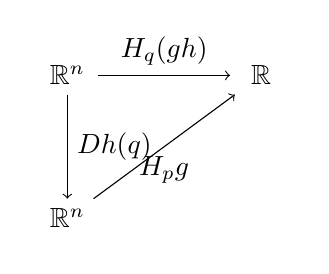
\begin{tikzpicture}
  \matrix (m) [matrix of math nodes, row sep=3.8em, column sep=4.8em, minimum width=2.2em]
  {
    \mathbb{R}^n & \mathbb{R} \\ 
     \mathbb{R}^n & \\ 
};
  \path[->]
  (m-1-1) edge node [above] {$H_q(gh) $} (m-1-2)
          edge node [auto] {$Dh(q) $} (m-2-1)
  (m-2-1) edge node [below] {$H_pg $} (m-1-2)
  ;
\end{tikzpicture}  

(quadratic) form $(H_pf)$ invariant under diffeomorphisms.


Let $C^2$ $f:M\to \mathbb{R}$.  \\
$\forall \,$ critical pt. $x$ of $f$, define \\
Hessian quadratic form
\[
\begin{aligned}
  & H_xf : M_x \to \mathbb{R} \\ 
  & H_xf : M_x \xrightarrow{ D\varphi_x } \mathbb{R}^n \xrightarrow{ H_{\varphi(x)}(f\varphi^{-1} ) } \mathbb{R}
\end{aligned}
\]
where $\varphi$ is any chart at $x$.

Thus, critical pt. of a $C^2$ real-valued function nondegenerate iff associated Hessian quadratic form is nondegenerate.  

Let $Q$ nondegenerate quadratic form on vector space $E$.

$Q$ negative definite on subspace $F \subset E$ if $Q(x)<0$ whenever $x\in F$ nonzero.

Index of $Q \equiv \text{Ind}Q$, is largest possible dim. of subspace on which $Q$ is negative definite.








cf. 1.1. Morse's Lemma of  Ch. 6, pp. 145, Morse Theory of Hirsch (1997) \cite{MHirsch1997}

\begin{lemma}[Morse's Lemma]
  Let $p\in M$ be nondegenerate critical pt. of index $k$ of $C^{r+2}$ map $f:M\to \mathbb{R}$, $1\leq r \leq \omega$.

  Then $\exists \, C^r$ chart $(\varphi,U)$ at $p$ s.t.
  \begin{equation}
    f\varphi^{-1}(u_1 \dots u_n) = f(p) - \sum_{i=1}^k u_i^2 + \sum_{i = k+1}^n u_i^2
  \end{equation}
  \end{lemma}

Let ${\,}^TQ \equiv Q^T$ denote tranpose of matrix $Q$.

\begin{lemma}
  Let $A = \text{diag}\lbrace a_1 , \dots , a_n \rbrace$ diagonal $n\times n$ matrix, with diagonal entries $\pm 1$.

  Then $\exists \, $ neighborhood $N$ of $A$ in vector space of symmetric $n\times n$ matrices, $C^{\infty}$ map
  \begin{equation}
P:N \to GL(n,\mathbb{R})
  \end{equation}
  s.t. $P(A)=I$, and if $P(B) = Q$, then $Q^T BQ = A$
\end{lemma}

\begin{proof}
  Let $B = [b_{ij}]$ be symmetri matrix near $A$ s.t. $b{11} \neq 0$ and $b_{11}$ has same sign as $a_1$.

    Consider $x=Ty$ where
    \[
\begin{aligned}
&  x_1 = \left[ y_1 - \frac{b_{12}}{b_{11}} y_2 - \dots - \frac{b_{1n}}{b_{11}} y_n \right] / \sqrt{ |b_n | } \\ 
& x_k = y_k \text{ for } k = 2, \dots n 
  \end{aligned}
    \]
  \end{proof}






\end{multicols*}

\begin{thebibliography}{9}


\bibitem{JLee2009}
Jeffrey M. Lee. \textbf{Manifolds and Differential Geometry}, \emph{Graduate Studies in Mathematics} Volume: 107, American Mathematical Society, 2009. ISBN-13: 978-0-8218-4815-9

\bibitem{JLee2012}
John Lee, \textbf{Introduction to Smooth Manifolds} (Graduate Texts in Mathematics, Vol. 218), 2nd edition, Springer,  2012, ISBN-13: 978-1441999818

\bibitem{VGuilleminAPollack2010}
Victor Guillemin, Alan Pollack. \textbf{Differential Topology}. American Mathematical Society. 2010. ISBN-13: 978-0821851937
\url{https://www.google.com/url?sa=t&rct=j&q=&esrc=s&source=web&cd=2&cad=rja&uact=8&ved=0ahUKEwjG96q9z63JAhWMLYgKHempDoMQFggmMAE&url=http\%3A\%2F\%2Fwww.mat.unimi.it\%2Fusers\%2Fdedo\%2Ftop\%2520diff\%2FGuillemin-Pollack_Differential\%2520topology.pdf&usg=AFQjCNF5imOH5xeXRSK60qzM7zT97sdIsw}

\bibitem{AShastri2011}
Anant R. Shastri. \textbf{Elements of Differential Topology}. CRC Press. 2011. ISBN-13: 978-0415339209

\bibitem{MHirsch1997}
Morris W. Hirsch, \textbf{Differential Topology} (Graduate Texts in Mathematics), Graduate Texts in Mathematics (Book 33), Springer (September 16, 1997). ISBN-13: 978-0387901480

\bibitem{Pras1996}
Agostino Pr\'{a}staro.  \textbf{Geometry of PDEs and Mechanics}.  World Scientific Publishing Co.  1996.  QC125.2.P73 1996  530.1'55353--dc20.  

Agostino Pr\'{a}staro.  \emph{Dipartimento di Metodi e Modelli Matematici per le Scienze Applicate, Universit\`{a} degli Studi di Roma ``La Sapienza''}.  

\bibitem{Kopp2010}
  Clemens Koppensteiner.  \emph{Complex Manifolds: Lecture Notes}.  \url{http://www.caramdir.at/uploads/math/piii-cm/complex-manifolds.pdf}
  

\bibitem{Vand2008}
Stefan Vandoren. \textbf{Lectures on Riemannian Geometry, Part II: Complex Manifolds}.  \url{http://www.staff.science.uu.nl/~vando101/MRIlectures.pdf} 

\bibitem{Hori2003}
Kentaro Hori (Author, Editor), Sheldon Katz (Editor), Albrecht Klemm (Editor), Rahul Pandharipande (Editor), Richard Thomas (Editor), Cumrun Vafa (Editor), Ravi Vakil (Editor), Eric Zaslow (Editor).  \textbf{Mirror Symmetry} (Clay Mathematics Monographs, V. 1).  Clay Mathematics Monographs (Book 1).  American Mathematical Society (August 19, 2003).  ISBN-10: 0821829556  ISBN-13: 978-0821829554  \url{https://web.archive.org/web/20060919020706/http://math.stanford.edu/~vakil/files/mirrorfinal.pdf}




\end{thebibliography}


\end{document}
